% ============================================================================
% REQUIRED PACKAGES & CONFIGURATIONS FOR COMPILING THIS EXPERIMENT:
% ----------------------------------------------------------------------------
% \usepackage{circuitikz}      % For drawing op-amp and RC oscillator schematics
% \usepackage{pgfplots}        % For plotting sine waves and phase shifts
% \pgfplotsset{compat=1.18}    % Ensures modern rendering engine defaults
% \usepackage{booktabs}        % For publication-grade tables
% \usepackage{amsmath}         % For mathematical equations
% \usepackage{siunitx}         % For standard units (\SI, \kilo\omega, \nano\farad)
% ============================================================================

\chapter{RC Phase Shift Oscillator}

\section{Aim}
To design, construct, and test an Op-Amp based RC Phase Shift Oscillator using IC 741. %The specific objectives are:
%\begin{enumerate}
%	\item To design an RC phase shift feedback network for a target oscillation frequency ($f_0 = 1\text{ kHz}$).
%	\item To set up the inverting amplifier gain to satisfy the Barkhausen criterion for sustained oscillations ($|A\beta| \ge 1$).
%	\item To measure the experimental frequency of oscillation and compare it with theoretical calculations.
%	\item To observe the phase shift introduced across each individual RC stage using a Digital Storage Oscilloscope (DSO).
%\end{enumerate}

\section{Pre-Lab Assignment}
Before coming to the laboratory, complete the following analytical tasks:
\begin{enumerate}
	\item Derive the overall transfer function $\beta(s) = \frac{V_{feedback}(s)}{V_{out}(s)}$ for a 3-section high-pass RC ladder network.
	\item Show that the frequency at which the total phase shift of the 3-stage RC network equals $180^\circ$ is given by:
	\begin{equation}
		f_0 = \frac{1}{2\pi R C \sqrt{6}}
	\end{equation}
	\item Prove that at the frequency of oscillation $f_0$, the attenuation factor of the feedback network is $\beta = \frac{1}{29}$, requiring an inverting amplifier gain magnitude of $|A_v| \ge 29$.
	\item Calculate the required value of $R_f$ for sustained oscillations if $R = 6.8\text{ k}\Omega$ and $C = 10\text{ nF}$.
\end{enumerate}

\section{Components and Equipment Required}
The required components and equipment for this experiment are listed in Table \ref{tab:components_rc_osc}.

\begin{table}[h!]
	\centering
	\caption{Components and Equipment Specifications}
	\label{tab:components_rc_osc}
	\begin{tabular}{llll}
		\toprule
		\textbf{S. No.} & \textbf{Item Name} & \textbf{Specification / Range} & \textbf{Quantity} \\
		\midrule
		1 & Operational Amplifier & IC 741 (8-pin DIP) & 1 No. \\
		2 & Resistors ($R$) & \SI{6.8}{\kilo\Omega} (1\% Tolerance) & 3 Nos. \\
		3 & Capacitors ($C$) & \SI{10}{\nano\farad} (Ceramic/Film) & 3 Nos. \\
		4 & Potentiometer ($R_f$) & \SI{500}{\kilo\Omega} (Linear Pot) & 1 No. \\
		5 & Fixed Resistor ($R_{f,\text{min}}$) & \SI{100}{\kilo\Omega} & 1 No. \\
		6 & Dual DC Power Supply & $\pm 15\text{ V}$ & 1 No. \\
		7 & Digital Storage Oscilloscope & Dual Channel, \SI{20}{\mega\hertz} or higher & 1 No. \\
		8 & Digital Multimeter (DMM) & $4\frac{1}{2}$ Digit & 1 No. \\
		9 & Breadboard \& Wires & Standard setup & As required \\
		\bottomrule
	\end{tabular}
\end{table}

\section{Theory}
An oscillator is an electronic circuit that converts a DC power supply voltage into a continuous, self-sustaining AC output signal without requiring any external AC input signal.

\subsection{Barkhausen Criterion for Oscillation}
For a feedback circuit to generate continuous sinusoidal oscillations at a specific frequency $f_0$, it must satisfy two fundamental conditions known as the Barkhausen Criterion:
\begin{enumerate}
	\item \textbf{Loop Gain Magnitude:} The magnitude of the overall loop gain must be greater than or equal to unity:
	\begin{equation}
		|A \cdot \beta| \ge 1
	\end{equation}
	\item \textbf{Loop Phase Shift:} The total phase shift around the feedback loop must be $0^\circ$ or an integer multiple of $360^\circ$:
	\begin{equation}
		\angle (A \cdot \beta) = 0^\circ \quad \text{or} \quad 360^\circ
	\end{equation}
\end{enumerate}

\subsection{Circuit Operation}
The RC Phase Shift Oscillator consists of an inverting amplifier stage and a 3-section high-pass RC feedback network:
\begin{itemize}
	\item \textbf{Inverting Amplifier Stage:} The op-amp is configured as an inverting amplifier, providing an inherent $180^\circ$ phase shift between its input (pin 2) and output (pin 6).
	\item \textbf{RC Feedback Network:} The feedback network consists of three identical cascaded RC high-pass sections. At the frequency of oscillation $f_0$, the three RC sections contributes a total feedback phase shift of $180^\circ$.
\end{itemize}

Combining the $180^\circ$ phase shift from the inverting op-amp with the $180^\circ$ phase shift from the RC network results in a total loop phase shift of $360^\circ$ ($0^\circ$), satisfying the Barkhausen phase condition.

At $f_0$, the 3-section RC ladder attenuates the signal by a factor of $\beta = \frac{1}{29}$. To overcome this loss and maintain $|A\beta| = 1$, the inverting op-amp voltage gain must satisfy:
\begin{equation}
	|A_v| = \frac{R_f}{R_3} \ge 29 \implies R_f \ge 29 \cdot R
\end{equation}

\section{Circuit Diagram}
The schematic for the Op-Amp RC Phase Shift Oscillator is shown in Figure \ref{fig:rc_osc_circuit}.

\begin{figure}[h!]
	\centering
	\begin{circuitikz}[scale=0.9, line width=0.8pt, transform shape]
		% Op-Amp IC 741
		\draw (0,0) node[op amp] (opamp) {IC 741};
		
		% Pin numbers
		\node[font=\small, above right] at (opamp.-) {2};
		\node[font=\small, below right] at (opamp.+) {3};
		\node[font=\small, above left]  at (opamp.out) {6};
		\node[font=\small, above right] at (opamp.up) {7};
		\node[font=\small, below right] at (opamp.down) {4};
		
		% Non-inverting input to ground
		\draw (opamp.+) -- ++(-0.5,0) node[ground] {};
		
		% Output node
		\draw (opamp.out) -- (1.5,0) node[circle, fill, inner sep=1.5pt] (outNode) {};
		\draw (outNode) -- (2.5,0) node[right] {$V_{out}$};
		
		% Feedback loop down
		\draw (outNode) -- (1.5,-2.5) 
		to[C, l_=$C_1\ (\SI{10}{\nano\farad})$, *-*] (-1.0,-2.5) node[circle, fill, inner sep=1.5pt] (nodeA) {}
		to[C, l_=$C_2\ (\SI{10}{\nano\farad})$, *-*] (-3.5,-2.5) node[circle, fill, inner sep=1.5pt] (nodeB) {}
		to[C, l_=$C_3\ (\SI{10}{\nano\farad})$, *-*] (-6.0,-2.5) node[circle, fill, inner sep=1.5pt] (nodeC) {};
		
		% Resistors to ground in RC network
		\draw (nodeA) to[R, l=$R_1\ (\SI{6.8}{\kilo\Omega})$] (-1.0,-4.5) node[ground] {};
		\draw (nodeB) to[R, l=$R_2\ (\SI{6.8}{\kilo\Omega})$] (-3.5,-4.5) node[ground] {};
		
		% Node C into Series R3 and then into Pin 2
		\draw (nodeC) to[R, l=$R_3\ (\SI{6.8}{\kilo\Omega})$] (-6.0, 0.5) -- (opamp.-);
		
		% Feedback Resistor Rf
		\draw (-1.5,0.5) node[circle, fill, inner sep=1.5pt] {} -- (-1.5,2.2)
		to[pR, l=$R_f\ (\text{Pot } \SI{270}{\kilo\Omega})$, name=myPot] (1.5,2.2) -- (1.5,0);
		\draw(myPot.wiper) to[short] ++(1.5,0);
		\draw (1.5,0) to[short] (1.5,2.75);
		% Vertical Power Lines
		\draw (opamp.down) -- ++(0, -0.8) node[right] {$-15\text{ V}$};
		\draw (opamp.up) -- ++(0, 0.6) node[right] {$+15\text{ V}$};
		
		
		% Node Labels for intermediate phase measurements
		\node[font=\small, above] at (nodeA) {$V_A$};
		\node[font=\small, above] at (nodeB) {$V_B$};
		\node[font=\small, left]  at (nodeC) {$V_C$};

	\end{circuitikz}
	\caption{Op-Amp RC Phase Shift Oscillator Circuit Schematic}
	\label{fig:rc_osc_circuit}
\end{figure}

\section{Design}
\subsection{Target Specifications}
\begin{itemize}
	\item Target Oscillation Frequency: $f_0 = 1\text{ kHz}$
	\item Op-Amp Power Supply: $V_{CC} = +15\text{ V}$, $V_{EE} = -15\text{ V}$
\end{itemize}

\subsection{Component Selection}
\begin{enumerate}
	\item Select a standard capacitor value: $C_1=C_2=C_3=C = \SI{10}{\nano\farad} = 10^{-8}\text{ F}$.
	\item Calculate the required resistance $R$ using the theoretical frequency formula:
	\begin{equation}
		f_0 = \frac{1}{2\pi R C \sqrt{6}} \implies R = \frac{1}{2\pi f_0 C \sqrt{6}}
	\end{equation}
	\begin{equation}
		R = \frac{1}{2\pi \times 1000\text{ Hz} \times (10 \times 10^{-9}\text{ F}) \times 2.4495} \approx \SI{6.497}{\kilo\Omega}
	\end{equation}
	Select the closest standard precision resistor value: $R_1 = R_2 = R_3 = R = \SI{6.8}{\kilo\Omega}$.
	
	\item Recalculate the theoretical frequency using standard component values:
	\begin{equation}
		f_{0,\text{theoretical}} = \frac{1}{2\pi \times (6.8 \times 10^3) \times (10 \times 10^{-9}) \times 2.4495} \approx \SI{955.4}{\text{Hz}}
	\end{equation}
	
	\item Calculate minimum feedback resistance $R_f$ for gain requirement ($|A_v| \ge 29$):
	\begin{equation}
		R_{f,\text{min}} = 29 \times R = 29 \times \SI{6.8}{\kilo\Omega} = \SI{197.2}{\kilo\Omega}
	\end{equation}
	Select $R_f$ as a combination of a \SI{180}{\kilo\Omega} fixed resistor in series with a \SI{22}{\kilo\Omega} potentiometer, or use a single \SI{270}{\kilo\Omega} variable potentiometer to allow smooth gain tuning.
\end{enumerate}

\section{Procedure}
Assemble the RC Phase Shift Oscillator circuit on the breadboard according to Figure \ref{fig:rc_osc_circuit}, and connect the power supply.
	%\item Connect the dual power supply ($\pm 15\text{ V}$) to pins 7 and 4 of IC 741.
	%\item Connect Channel 1 of the DSO to $V_{out}$ (pin 6).
Slowly adjust the feedback potentiometer $R_f$ starting from a low resistance until a stable, undistorted sine wave is obtained.
%	\begin{itemize}
%		\item Observe that for $R_f < 197.2\text{ k}\Omega$, oscillations decay to zero.
%		\item Increase $R_f$ until stable, continuous sinusoidal oscillations appear on the DSO.
%		\item Observe that if $R_f$ is set too high, the waveform clips near the power supply saturation rails ($\approx \pm 13.5\text{ V}$). Fine-tune $R_f$ for a clean, undistorted sine wave.
%	\end{itemize}
Measure the frequency $f_0$ and peak-to-peak amplitude $V_{p-p}$ of $V_{out}$ on the DSO. %Observe the signals at node $V_A$, node $V_B$, and node $V_C$ and measure the phase angle shift introduced by each RC stage relative to output node $V_{out}$.

\section{Precautions}
\begin{enumerate}
	\item Ensure correct power supply polarity ($\pm 15\text{ V}$) before turning on the power supply to prevent destroying the IC.
	%\item Avoid excessive feedback resistance ($R_f$) setting to minimize severe harmonic distortion and flat-top waveform clipping.
	\item Keep component leads and wiring short to reduce stray parasitics.
\end{enumerate}

\section{Model Graph / Expected Waveforms}
Figure \ref{fig:osc_waveforms} shows the expected time-domain sinusoidal output along with intermediate phase-shifted signals across the RC network stages.

\begin{figure}[h!]
	\centering
	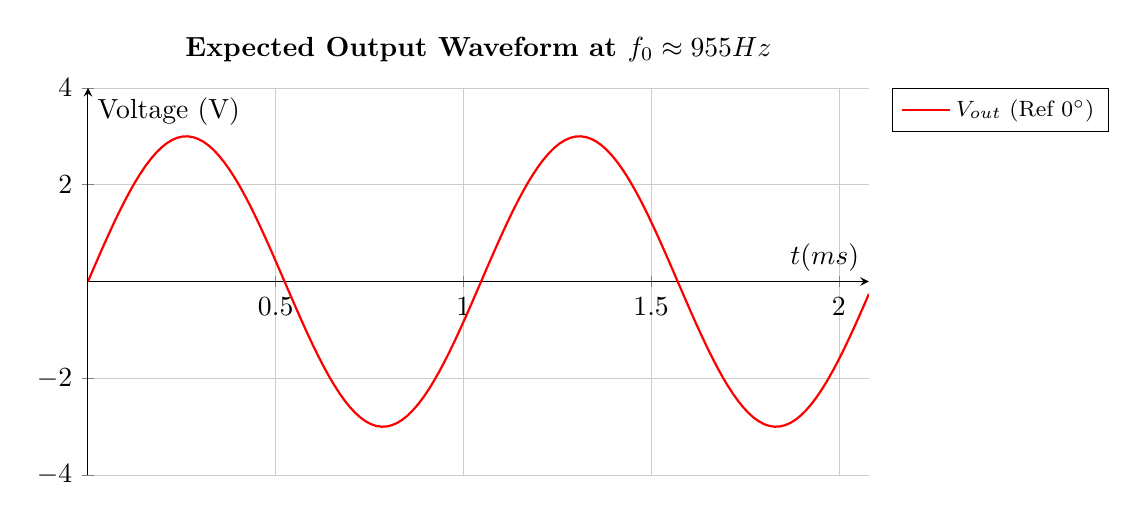
\begin{tikzpicture}
		\begin{axis}[
			axis lines=middle,
			xlabel={$t\text{ (ms)}$},
			ylabel={Voltage (V)},
			xmin=0, xmax=2.08,
			ymin=-4, ymax=4,
			xtick={0,0.5,1.0,1.5,2.0},
			grid=both,
			grid style={line width=.1pt, draw=gray!20},
			major grid style={line width=.2pt, draw=gray!40},
			width=11.5cm, height=6.5cm,
			title={\textbf{Expected Output Waveform at $f_0 \approx 955\text{ Hz}$}},
			legend pos=outer north east,
			legend style={font=\footnotesize}
			]
			% Vout (Pin 6)
			\addplot[thick, red, domain=0:2.08, samples=150] {3.0*sin(deg(2*pi*0.955*x))};
			\addlegendentry{$V_{out}$ (Ref $0^\circ$)}
			
			% Node A (Shifted by 60 deg)
%			\addplot[thick, blue, dashed, domain=0:3, samples=150] {2.0*sin(deg(2*pi*1*x + 60))};
%			\addlegendentry{$V_A$ ($+60^\circ$)}
			
			% Node B (Shifted by 120 deg)
%			\addplot[thick, green!60!black, dashdotted, domain=0:3, samples=150] {1.2*sin(deg(2*pi*1*x + 120))};
%			\addlegendentry{$V_B$ ($+120^\circ$)}
			
			% Node C (Shifted by 180 deg)
%			\addplot[thick, magenta, dotted, domain=0:3, samples=150] {0.6*sin(deg(2*pi*1*x + 180))};
%			\addlegendentry{$V_C$ ($+180^\circ$)}
		\end{axis}
	\end{tikzpicture}
	\caption{Output Signal}
	\label{fig:osc_waveforms}
\end{figure}

%\section{Observation Table}

%\subsection{Oscillation Frequency Measurement}
%Record the experimental frequency measurements in Table \ref{tab:freq_obs}.

%\begin{table}[h!]
%	\centering
%	\caption{Theoretical vs Practical Oscillation Frequency}
%	\label{tab:freq_obs}
%	\begin{tabular}{cccccc}
%		\toprule
%		\textbf{Calculated } $R$ & \textbf{Capacitance } $C$ & \textbf{Theoretical } $f_0$ & \textbf{Measured Period } $T_0$ & \textbf{Practical } $f_0$ & \textbf{\% Error} \\
%		\midrule
%		\SI{6.8}{\kilo\Omega} & \SI{10}{\nano\farad} & \SI{955.4}{\text{Hz}} & & & \\
%		\bottomrule
%	\end{tabular}
%\end{table}

%\subsection{Phase Shift across Feedback Stages}
%Record the phase angles measured relative to $V_{out}$ in Table \ref{tab:phase_obs}.
%
%\begin{table}[h!]
%	\centering
%	\caption{Phase Shift Measurements Across RC Ladder}
%	\label{tab:phase_obs}
%	\begin{tabular}{lcccc}
%		\toprule
%		\textbf{Test Node} & \textbf{Theoretical Phase Shift} & \textbf{Measured Time Lag } $\Delta t$ & \textbf{Measured Phase Shift } $\theta$ & \textbf{Status} \\
%		\midrule
%		Node $V_A$ (Stage 1) & $60^\circ$  & & & \\
%		Node $V_B$ (Stage 2) & $120^\circ$ & & & \\
%		Node $V_C$ (Stage 3) & $180^\circ$ & & & \\
%		\bottomrule
%	\end{tabular}
%\end{table}

\section{Result}
The RC Phase Shift Oscillator using IC 741 was successfully designed, constructed, and tested:
\begin{itemize}
	\item Continuous sinusoidal oscillations were obtained at an experimental frequency of $f_{0,\text{practical}} = \rule{2cm}{0.15mm}\text{ Hz}$, compared to the theoretical value of \SI{955.4}{\text{Hz}} %(Percentage Error: \rule{1.5cm}{0.15mm}\%).
%	\item The critical gain requirement ($R_f \ge 29 R$) and $180^\circ$ feedback phase shift condition were experimentally verified.
\end{itemize}

\section{Questions}
\begin{enumerate}
	\item Why is an RC phase shift oscillator unsuitable for generating high radio frequencies (RF)?
	\item What is the effect on the oscillation frequency if all resistor values in the RC feedback network are doubled?
	\item Why does an RC phase shift oscillator require at least three RC stages rather than two stages to produce sinusoidal oscillations?
	\item Explain how auto-gain control (AGC) or diode limiters can be added to the feedback loop to stabilize the amplitude of oscillations without waveform clipping.
	\item Compare the frequency stability and output amplitude stability of an RC phase shift oscillator with a Wien Bridge oscillator.
\end{enumerate}